\providecommand{\mainpath}{..} % Command to retrieve the path of the main file. It must be defined before documentclass.

\documentclass[\mainpath/main]{subfiles}
\begin{document}

\chapter{Architectural Design}
\label{architectural_design}

% Command to be executed after the starting of every chapter
\setmyfancystyle
% ----------------

In this chapter the complete architecture of myTaxiService is shown with various levels of description. In the \autoref{ArchitecturalDesign:high_level} there is a global view and the interactions between all the components are described.\\ 
The data tier is illustrated in \autoref{ArchitecturalDesign:component} with all related policies and entities. Then the other tiers are characterized using different diagrams.\\
In the \autoref{ArchitecturalDesign:deploy} the deployment of each components is illustrated (for instance the data component is sit in a different place with respect to the other component? It is replaced twice or more? And similar question will have an answer).\\
In \autoref{ArchitecturalDesign:runtime} the view level is defined. The interactions between all kinds of user and the system are described using UX diagrams and sequence diagrams that display the order in which each screen is visualized. Besides, the mockups of these screens are shown in %\autoref{UI}.
\\
A standalone paragraph, the \autoref{ArchitecturalDesign:comp_interfaces}, is dedicated to list all interfaces, both internal (between two components) and external.\\
Finally, in the \autoref{ArchitecturalDesign:design_patterns} the design patterns used to develop myTaxiService are described first in general case. After that, all the changes needed to adapt this design patterns to our system are characterized.


\section{Distinctions between various kind of Users and Clients}
\label{ArchitecturalDesign:preamble}
The "visible architecture" of myTaxiService is very varied. The term visible is referred to various user interfaces, so what the users can see when they are using the system.\\
On the other hand, we have said that myTaxiService is varied because it has two principal version (MA and WS) and for both of them there are a few levels of specialization, according to the kind of the user. All of them are explained in this paragraph.\\
\\
The WS version is shown into a browser, so there is no client application that can be used. Hence, all the pages are loaded into the server and then they are sent to the client browser.\\
Instead, the MA is a client application and it has different ways to communicate with the server. All the aspects concerning these differences are explained better during the descriptions of the architecture's components that handle the clients.\\
\\
%Fare un riferimento al capitolo che mette in relazione RASD e DD per far capire il tipo di attore?
The cab company is the special user who administrates the service. Obviously, it has a command center at its headquarters where it can control both the system and the service situation. Hence its special functions are not implemented neither in the MA nor in the WS, but they can directly access the server using private keys and reserved terminals.\\
A customers can use both the MA and the WS to enjoy his functionalities. No particular cases or restriction are reserved to them.\\
When a driver logs into the service, we suppose that it is working, so his special functionalities are developed and implemented only for the MA. In fact no driver carries a computer with an internet connection on his taxi and uses it. On the other hand, since the driver is also an user, it can use the WS, but here he has only the user functionalities due to the reason shown above.\\



\section{High level components and their interaction}
\label{ArchitecturalDesign:high_level}

The main structure of myTaxiService can be described as a Service-Oriented architecture (see \autoref{ArchitecturalDesign:design_patterns} to have a detailed description of this design pattern). In addition to this idea the Model-View-Control paradigm is applied in order to develop a good-programmed, a reusable and a easy-maintainable system.
\begin{figure}[h]
	\centering
	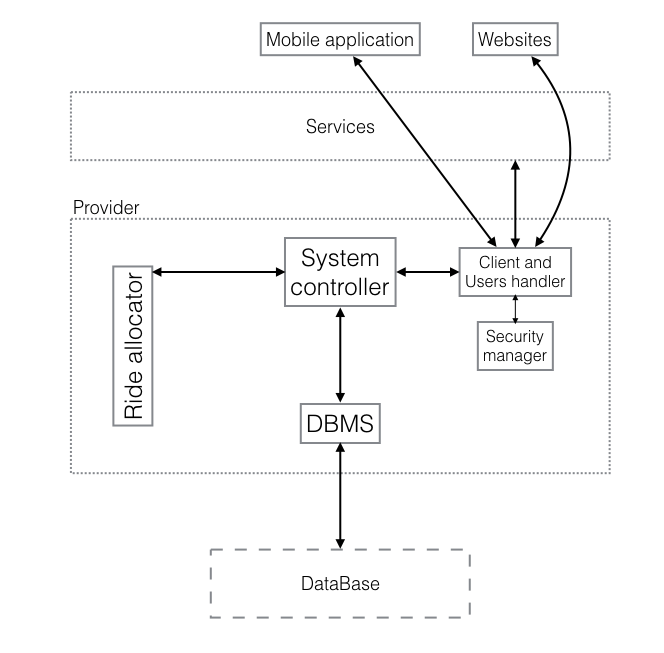
\includegraphics[width=15cm] {main_architecture}
\end{figure}


TESTO NON UFFICIALE\\
Fare qui un mega diagramma component che illustra le relazioni tra i vari componenti del nostro sistema. Architectures with three main components: data tier, server tier (split into 
various components, like manager of DB, security controller, client handler, ... we have to decide all of this component) and client tier that not contain the client applications, but the component which interacts with the client application, sends the pages, and makes a first check on data received by user (then the homonymous component into the server tier handles all the available actions).. 

Descrizione precisa delle interazioni\\


\section{Component view}
\label{ArchitecturalDesign:component}

TESTO NON UFFICIALE\\
qui si descrivono nel dettaglio tutti i vari componenti, specialmente il data tier e il server tier. 

\section{Deployment view}
\label{ArchitecturalDesign:deploy}

$TESTO NON UFFICIALE\\
Distribuzione dei vari component\\
Ci sono più macchine per il server? Ci sono altri componenti come firewall? ecc$

\section{Runtime view}
\label{ArchitecturalDesign:runtime}

TESTO NON UFFICIALE\\
qui si pone particolare attenzione alle screen e quindi al client tier.\\
Tutti i sequence diagram e gli UX saranno messi qui\\

\section{Component Interfaces}
\label{ArchitecturalDesign:comp_interfaces}

TESTO NON UFFICIALE\\
descrizione di tutte le interfacce tra i vari component e verso l'esterno.\\
Forse si metteranno anche i principali metodi?\\


\section{Selected architectural styles and patterns}
\label{ArchitecturalDesign:design_patterns}


EVENTBASED per ora\\


%End of chapter
\end{document}